\documentclass[]{article}

\usepackage{graphicx}

%opening
\title{Figures for  3-D printed oxygen devices}
\author{}

\begin{document}

%\maketitle

\section{figures}

\begin{figure}[H]
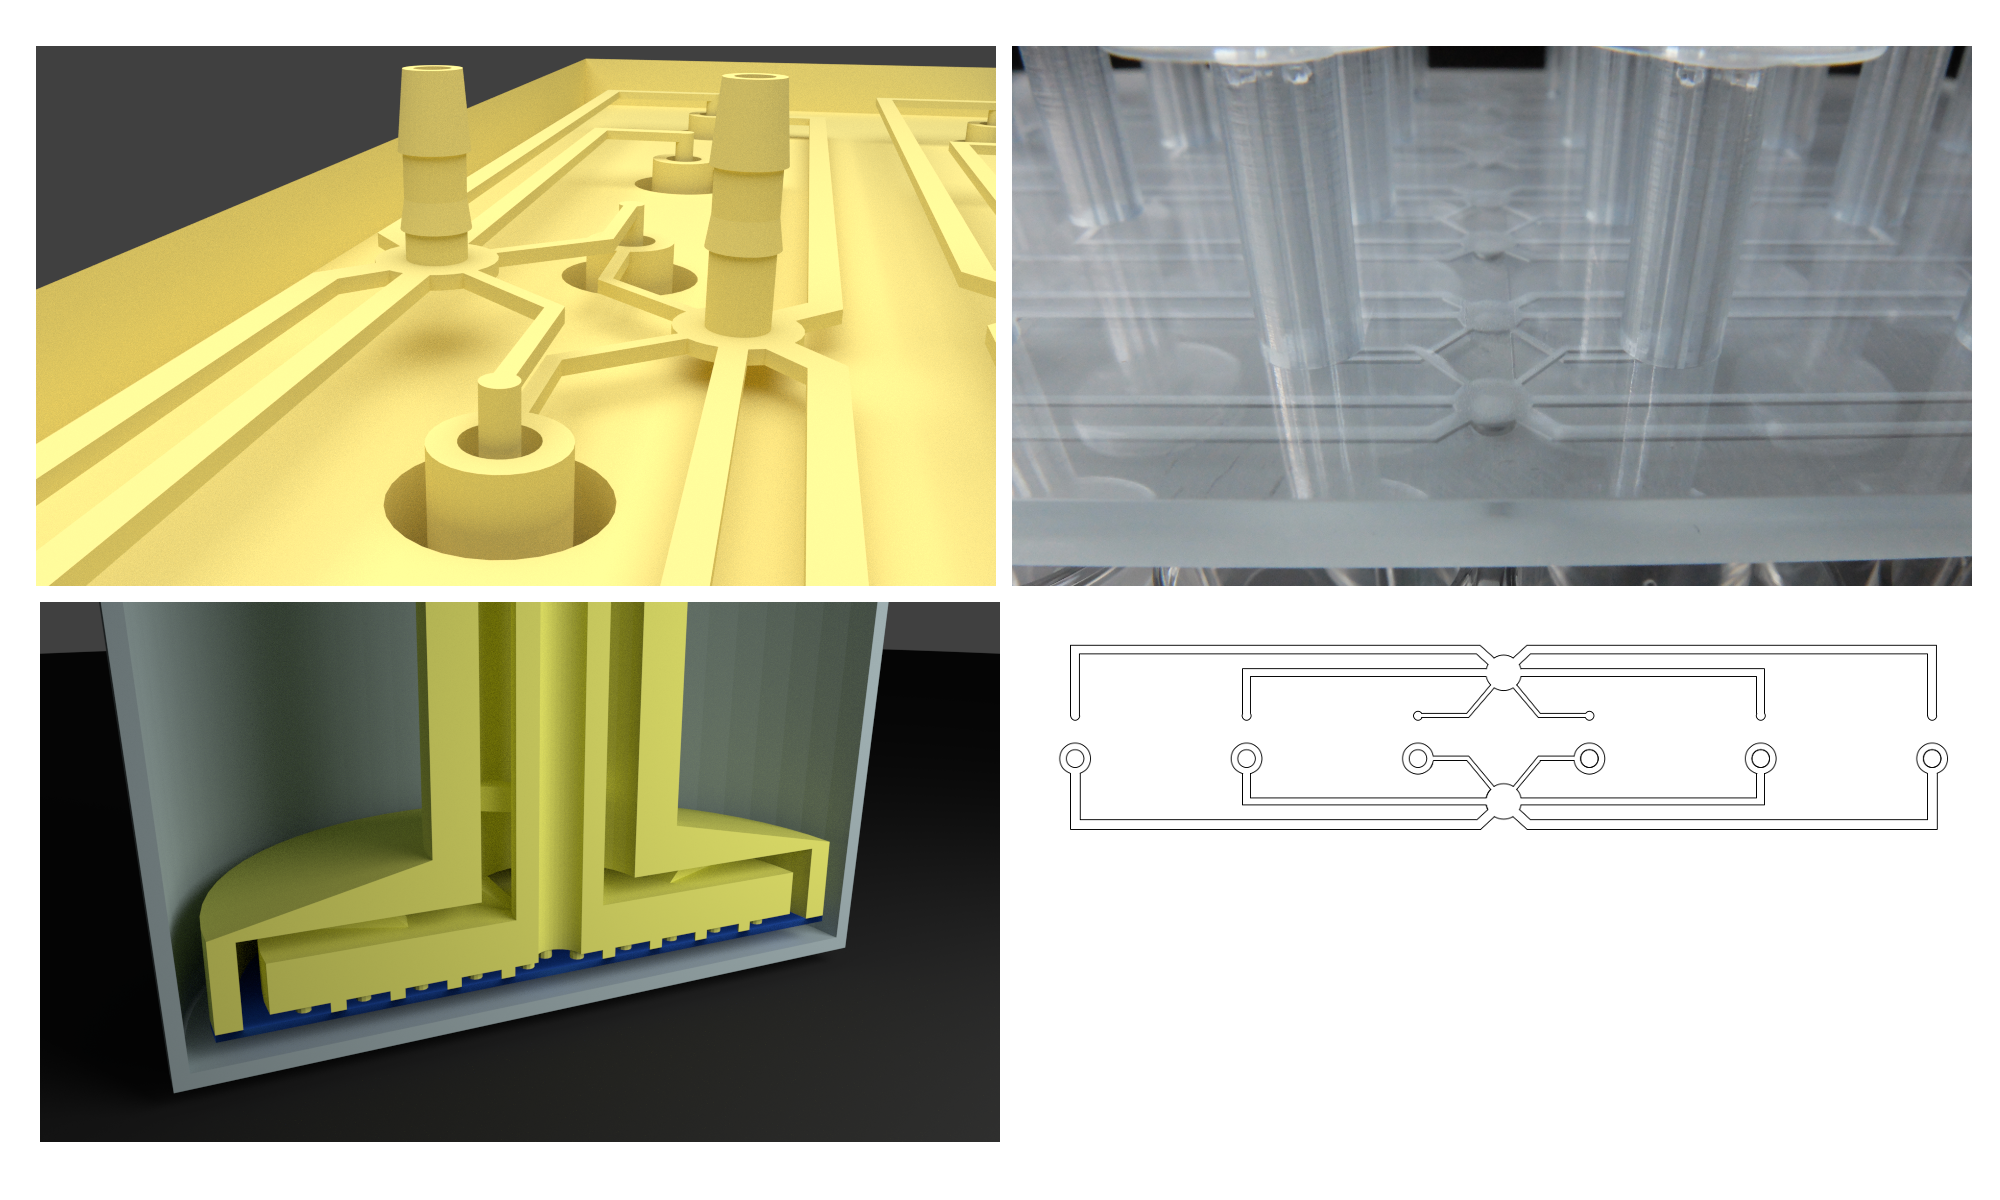
\includegraphics[scale=0.2]{fig1.png} 
\caption{
{\bf Design of 24-well Insert Device.}
(A) Rendering of whole 3D printed part.
The device inserts into a standard 24 well plate.
An inlet and oulet barb allows perfusion of gas to control 6 channels.
The design is iterated four times for a total of 24 wells.
(B) Cross-section demonstrating how the microfluidic distribution network and double pipes are connected. 
The two adjacent asymentical distribution networks are spaced 1 mm apart along the z axis allowing them to overlap and enter the seperate vertical pipes.
The arrows indicate the flow direction.
The incoming gas enters enters the outer pipe on its way to the bottom of the well and returns through the inner pipe.
(C) At the bottom of the pillar gas flow along the PDMS membrane (blue), which is supported by micropillars, and exits via the inner pipe.
Diffusion occurs rapidly through the PDMS membrane to the cell culture spaced 500 $\mu$m away at the bottom of the well.
(D) The width of the channels in the distribution network are such that the flow rates are equalized to each well dependent on the path length.
----The empty space above (D) will have labels and arrow pointing to: membrane, micropillars, supports, inner pipe, and outer pipe.----
}
\label{figure1}
\end{figure}

\begin{figure}[H]
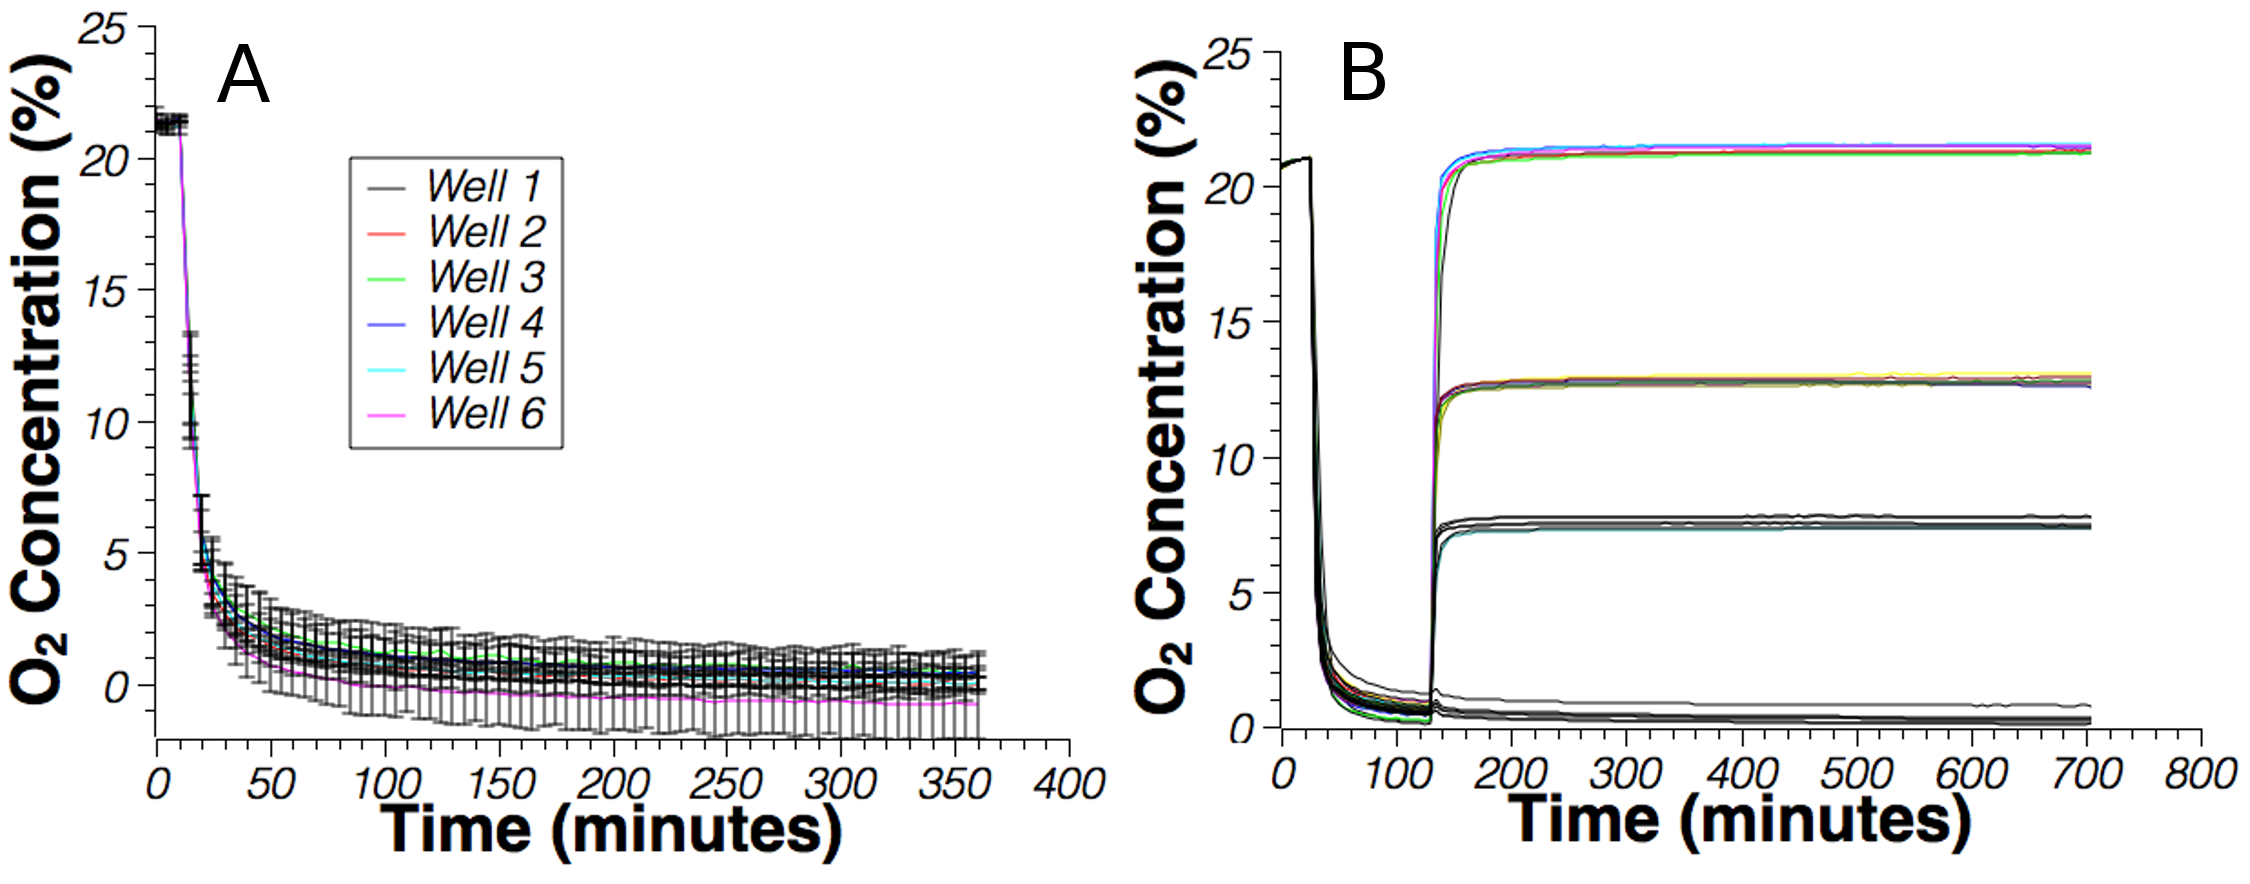
\includegraphics[scale=0.25]{fig2.png}
\caption{
{\bf Oxygen Characterization.}  Time course data of oxygen being evacuated from the culture area as 0\% oxygen gas is perfused through the device. Each 6 well row of the plate can be controlled independently.  
}
\label{figure2}
\end{figure}

\begin{figure}[H]
%\includegraphics[scale=0.2]{image.jpg} % remove for manuscript submission
\caption{
{\bf PCR Data.}  Not finished yet.  
}
\label{pcr-data}
\end{figure}

%\begin{abstract}

%\end{abstract}

%\section{}

\end{document}
